\section{The Action}

\ldots

\subsection{Disposition of Forces}

\ldots

\subsection{Opening moves}

\subsubsection{Americans:}

\begin{figure}[h]
    \begin{center}
    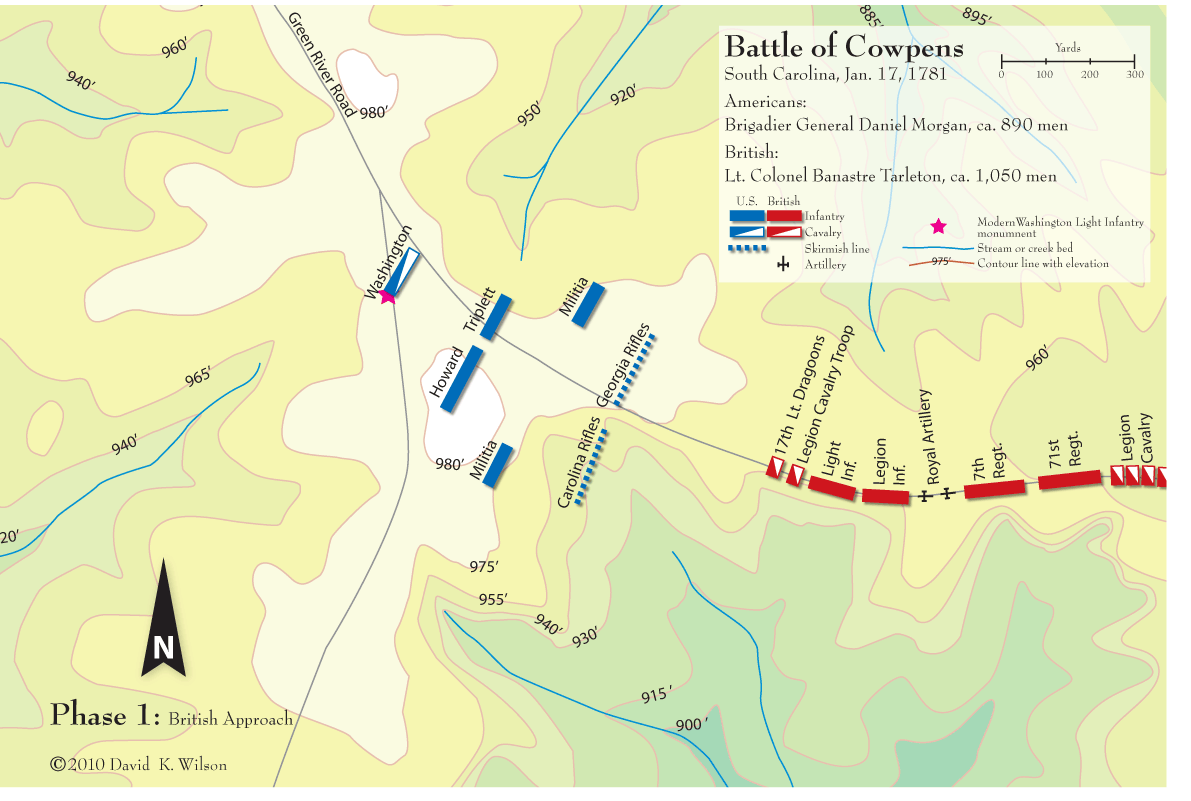
\includegraphics[width=\textwidth]{gfx/beiber01}
    \end{center}
    \caption{Initial disposition of the Armies.\cite{wilson_blogmap}}
    \label{beiber01}
\end{figure}
%\url{http://www.davidwilsonhome.com/homepage/Perspectives/Entries/2010/4/11_The_Battle_of_Cowpens__A_Cartographic_Interpretation.html}



Brigadier General Daniel Morgan, knowing that Tarleton was in full pursuit,
selected Cowpens as the field of battle.  He described his decision to fight
there in later correspondence with Nathanael Greene, “I would not have had a
swamp in the view of my militia on any consideration; they would have made for
it, and nothing could have detained them from it.  As to covering my wings, I
knew my adversary and was perfectly sure I should have nothing but downright
fighting.  As to retreat, it was the very thing I wished to cut off all hope of”
\cite[46]{moncure_cowpens_1996}.  Morgan chose the location for battle and anticipated
Tarleton's forces arriving the following day.  He had deployed reconnaissance
forces that would alert him when Tarleton approached and, knowing his men, used
the hours awaiting word of Tarleton's advance to align his forces.

Morgan had selected the time and place for battle.  As a result, he took full
use of this advantage over Tarleton in the night prior to the British advance:

\begin{quote}
  ``The night gave Morgan time to prepare his men for combat the next day, and
  the skilled leader made the most of his opportunity. Allowing his troops to
  prepare physically -- cleaning their weapons, eating and so forth -- he walked
  among them to prepare them emotionally for the horrors of eighteenth-century
  battle. Major Thomas Young of South Carolina wrote that Morgan showed a keen
  sense of how to command militia: `He went among the volunteers, helped them
  fix their swords, joked with them about their sweet-hearts, told them to keep
  in good spirits, and the hour would be ours'\,'' \cite[47]{moncure_cowpens_1996}
\end{quote}

After an evening of resting, rallying, and prepping the troops, Morgan spent the
early morning hours briefing his plan.  There is some discrepancy in reports as
to whether Morgan briefed his entire force or just key leadership, but the fact
remains that Morgan completed the task of briefing his plan to subordinates in
sufficient time and fashion in order to disseminate necessary information to his
entire force.   The task of occupying the defensive line was completed in the
early morning hours before light.  Few specific recollections exist regarding
the formal occupation of the American defensive lines, but this action most
likely occurred after the troops had been fully briefed.   Once the defense was
established, Morgan and his subordinate leaders spent their time continually
speaking with and rallying the troops. 

\begin{quote}
“Morgan rode his lines.  To the 120 Georgia and North Carolina skirmishers he
asked for courage and marksmanship, when the enemy was within firing distance.
They should then withdraw slowly; reloading and firing as they went, until they
rejoined their comrades in the militia line 150 yards behind them. ‘Let me see,’
he called out just before leaving them, ‘which are most entitled to the credit
of brave men, the boys of Carolina or those of Georgia.’ Then he rode back to
Andrew Pickens’s main line of militia and exhorted them to hold their fire until
the British were within fifty yards, to deliver two volleys, then follow the
plan by crossing to the left in front of Howard’s Continentals and gathering
just behind that main line of resistance.  He complimented them for past actions
and implored them to add to their gallant reputation.  On this occasion, he
said, they would not have to stand alone against regulars, for supporting them
were American regulars superior to the enemy’s.  To flee, Morgan told them,
would invite destruction” (Buchanan, p.320).
\end{quote}

Morgan was well aware of Tarleton's history, personality, and reputation as an
aggressive combatant.  His developed understanding of Tarleton's rash
personality and fierceness in combat led him to make assumptions regarding
Tarleton's actions.  Morgan used this knowledge of the British leader and
coupled it with his significant understanding of the troops under his own
command.  The result of Morgan’s analysis led to his choice of defense in
attempt to force Tarleton to act impulsively on the battlefield.  Morgan also
had an understanding of his troops.  He knew that the militiamen were
relatively untrained for combat and nervous facing such impressive formal
force.  He took advantage of this knowledge and created a defense that would
empower his inexperienced troops and coerce Tarleton into deploying his forces
in a non-advantageous sequence.   By the time Tarleton arrived on the field of
battle, Morgan and his troops were ready and waiting.  Morgan's leadership and
strong command and control of the situation resulted in a force that was ready
for the battle and men who possessed great confidence in their leadership.

\subsubsection{British:}

Tarleton had arrived in camp at Burr’s Mill on the 16th of January, one day
after Morgan and his troops had passed through that location.  Tarleton was
determined with pursuing the Americans and seizing the opportunity for battle.
The British arrived at this location in the late evening.   The troops were told
to rest and prepare for a fight the next day.  Tarleton spent his time focused
on pursuit and preparing for a fight.  “Tarleton’s men at Burr’s mill got what
sleep they could.  Tarleton continued to collect information and plan for the
next day.  He used his own Americans well … About midnight, scouts brought word
‘of a corps of mountaineers on the march from Green river.’ Tarleton mulled over
intelligence reports and planned his movements” (Babits p.56).  Tarleton took
this information from his scouts and seized the opportunity to advance on the
Americans.  He awoke his troops at around two o’clock and gave them the order to
prepare for movement.

On the morning of 17 January, at approximately three o’clock, Tarleton gave his
troops the order to advance.  Having pinpointed the Americans’ location and
under the belief that they were in full retreat, it was Tarleton’s intent to
make the roughly six mile movement and attack the Americans at first light.
Tarleton’s troops had arrived at this location only five hours earlier.  The
troops had very little to eat and were given a small amount of rest prior to the
movement.  This ground patrol took Tarleton’s troops from their location at
Morgan’s previous camp through freezing streams and dense thick brush in the
cold weather.  During this movement, the British troops would march up a reverse
slope, out of the thicket, and onto the field of battle.   Tarleton describes
the movement in a narrative:

\begin{quote}
 “Three companies of light infantry, supported by the legion infantry, formed
 the advance; the 7th regiment, the guns, and the 1st battalion of the 71st,
 composed the center’ and the cavalry and mounted infantry brought up the rear.
 The ground which the Americans had passed being broken, and much intersected by
 creeks and ravines, the march of the British troops during the darkness was
 exceedingly slow, on account of the time employed in examining the front and
 flanks as they proceeded”
 \cite[TAB Q, 14]{rauch_battle_2007}
\end{quote}

Following the crossing of Thicketty creek, Tarleton released an advanced
reconnaissance party of Cavalry with the express intent of locating Morgan’s
defense.  The troops rode forward and reported back Morgan’s location as well as
an estimate on the size of the American force.  Tarleton received this
information and drove forward.  There are many accounts by soldiers and
leadership alike that report this was not an easy movement.  The temperatures
were bitterly cold and, although Morgan's troops had passed through this same
path only a day earlier, there are reports of the British troops attempting to
set fire to the brush in order to blaze a path.   The first portion of the
movement was the most difficult as it took the men through brush until they
became close to Cowpens and were able to organize on Green River road.
Tarleton’s troops were on the hunt and although they were comprised mainly of
seasoned warfighters, it is likely that the long period of pursuit combined with
freezing temperatures, a short period or rest and preparation, and a difficult
movement were having their effect on the morale and physical readiness of his
troops.  Babits describes this movement, “By all accounts, the British had a
difficult time swimming horses and felling trees for bridges on this exhausting
march to contact.  Lieutenant Roderick MacKenzie, traveling with his light
infantry company, may have exaggerated, but crossing knee-deep streams in
January is hard on mind and body.” \cite[57]{babits_devil_2001}

After approximately four hours of movement, on the frozen morning of January 17,
1781, British Lieutenant Colonel Banastre Tarleton's disciplined group of
British soldiers broke through the wood line at Cowpens to face Brigadier
General Daniel Morgan and his group of Continental Army regulars and militia.
Upon breaking through the brush at Cowpens, Tarleton began to organize his
troops.  Tarleton’s recollection of this instance differs from that of his
troops, “According to Tarleton, he then directed his line to remove their packs
and to file to the right until the flank force faced its counterpart directly”
(Moncure, p.51).  The reality of Tarleton’s preparation on the battlefield was
later questioned by his subordinate leadership and is supported by their
recounts of the battle with a general consensus that,

\begin{quote}
  “He (Tarleton) did not wait until the Highlanders and his main body of
  cavalry, which he would hold in reserve, had gotten completely clear of the
  thick underbrush along Thicketty Creek.  Nor did he consult with his two
  veteran infantry commanders, Major Archibal McArthr of the Highlanders and
  Major Timothy Newmarsh of the Fusiliers.  Instead he formed his main line for
  an immediate general advance” (Buchanan, p.321)
\end{quote}


Regardless of the time which elapsed as Tarleton prepared his troops for battle,
they were observed by and faced with Morgan’s awaiting troops.  With the
American troops in sight, Tarleton ordered the British to drop their excess
equipment in order to be lighter for battle.  Morgan’s troops witnessed this
movement and act of British formal military procedure as the British line
organized and filed itself to the full length of the American Front.  British
Officers and their American opponents recalled this moment, “So impatient was
Tarleton that he ordered his main line forward before Major Newmarsh had
finished posting his officers.  There began the noise of an eighteen-century
battle.  The drum beat and the fifes shrilled.  Artillery boomed.  Officers and
sergeants bawled orders.  The British line, Morgan wrote in his battle report,
‘move on with the greatest impetuosity shouting as they advanced’“ (Buchanan,
p.321).   Morgan’s recollection of the British moving hastily as they occupied
their assault positions was likely an intimidating sight for the inexperienced
Americans on the front lines.   Many of the troops later recalled this event as
an intimidating display of force.

The movement and rapid occupation of the line were an exercise in British
military protocol.  Tarleton's forceful personality had already created
disruption amongst his troops and subordinate leadership.  He had maintained a
commanding presence on the battlefield, but lacked either the understanding or
insight necessary to prepare his troops mentally or physically.  Instead of
taking the precautions necessary during a deliberate attack, Tarleton's actions
were impulsive.  This impulsiveness and rush to battle without taking the
adequate precautions necessary was exactly what Morgan was expecting.


The British had established their line.  Tarleton had pressed them forward into
position for battle.  The men stood ready to fight, but were suffering from
physical exhaustion due to lack of sleep, food, and a difficult pursuit.  The
British troops would meet an organized force in Morgan’s men.  The Americans
were well rested and prepared for their attack.  Tarleton’s forcing of his
troops quickly into position to face an awaiting enemy without staging,
attending to priorities of work, or developing a plan was evident during the
onset of battle.  Tarleton’s demanding and potent leadership style got his
troops to the fight, but time would soon tell if it would be enough to will them
to a victory.  The small psychological advantage Tarleton gained through the
drill and ceremony as well as brute force of his troops would soon diminish with
the firing of the battle's first shots.

\begin{figure}[h]
    \begin{center}
    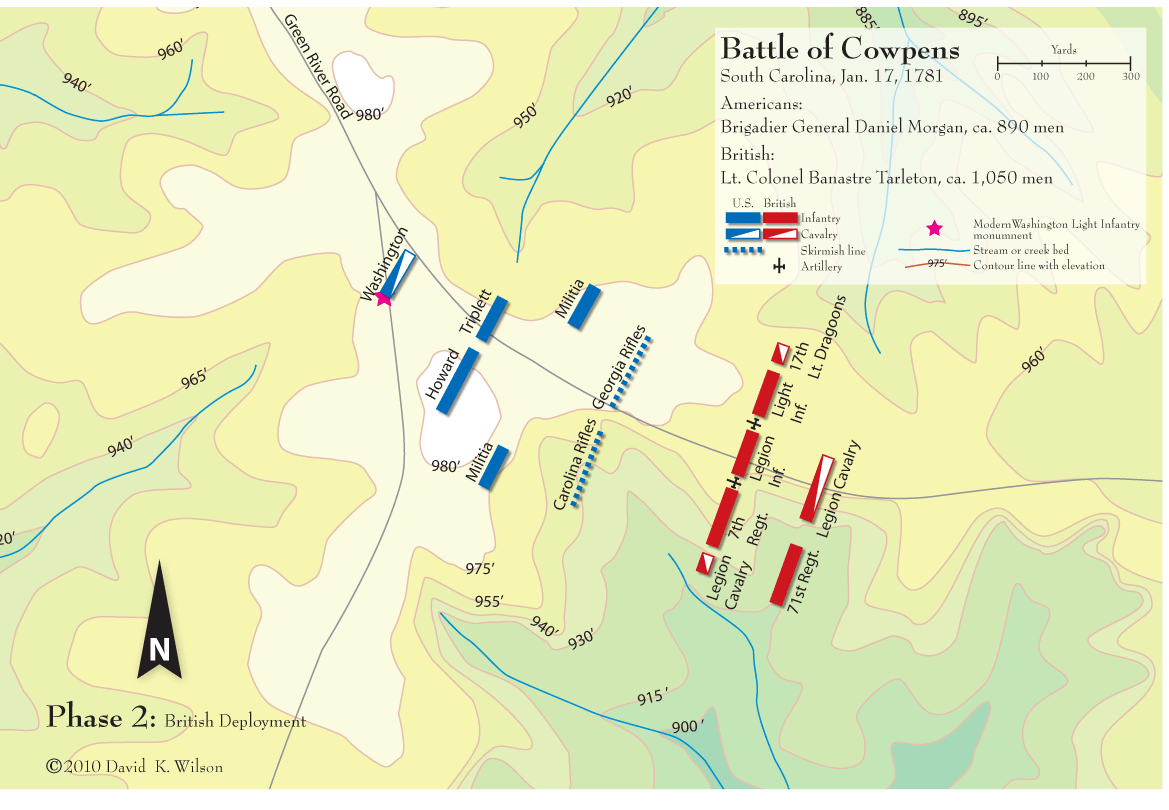
\includegraphics[width=\textwidth]{gfx/beiber02}
    \end{center}
    \caption{British Deployment at the battle of Cowpens \cite{wilson_blogmap}.}
    \label{terrain1}
\end{figure}


\subsubsection{Morgan's Troops Aligned for the Defense}

Brigadier General Morgan established a three line defense. Morgan's
troops were rested, well briefed, and roused for battle.  He had taken a full
“home field” advantage to use his developed knowledge of the backwoods and
understanding of his troops' abilities to emplace each unit in a role which
suited their strengths.  The North Carolina, South Carolina, and Georgia
sharpshooters were out in front, establishing a line of skirmishers intent upon
causing disruption at earliest opportunity.   Colonel Andrew Pickens four
battalions of Virginia militia were next.  The third and main line of defense
was the Continental Army along with Washington's cavalry held in reserve.

The Sharpshooters from the Southern States were placed approximately 300 meters
in front of the continental line (Moncure, p.48) and only a few hundred meters
in advance of the Virginians.  They would be emplaced in this position and
dispersed out amongst any trees and brush.   This action would force Tarleton to
react and leave him little ability to see what lay behind them.  The skirmishers
would take cover at this point and begin to engage the British at earliest
opportunity.  These men would be tasked to harassment fires with an intent to
disrupt British command and control therefore rushing the British into a rapid
decision making process.  These men were by no means meant to stand and fight.
As soon as the British began an advance or released their Cavalry in an expected
fashion, the skirmishers would fall back and reinforce the main line of the
militia.  This would serve another purpose which was the cornerstone of Morgan's
plan: deceive the British into believing that the American lines of defense were
breaking down into retreat.

The Virginia Militia, led by Colonel Andrew Pickens, was emplaced roughly 150
meters in front of the Continental troops' line.  These four battalions of men
from the Virginia militia knew their task well and it was with them that the
true battle would begin.  Reeling from their assault on the skirmishers, Morgan
assumed the British would organize and attack this line as if it were the main
body.  As a result, Morgan emplaced these men behind the skirmishers on level
ground.  The militia was tasked with holding their fire until the British came
within less than 100 meters.  At that time, they would fire three volleys into
the British line and fall back behind the continental troops led by Lieutenant
Colonel Howard.  This was meant to further exploit the British offensive with
aimed shots at the Officer and Non-Commissioned Officer leadership.  

The Delaware and Maryland Continental soldiers were led by Lieutenant Colonel
John Eager Howard.  Morgan emplaced these troops on slightly elevated terrain.
It was these troops who were tasked with facing and destroying the British
regulars.  These paid troops had seen combat and were prepared for battle.
Morgan’s knowledge of the British and of Tarleton specifically also led him to
this course of action.  It was his intent to cause the British to pursue the
fleeing militia men so that they met the Continental Army in an unorganized
state with an overwhelming mass of firepower.

Finally, Morgan placed the 3rd Continental Dragoons, led by Lieutenant Colonel
William Washington, as a reserve further behind the Continental Troops.  He
positioned these men out of sight of the British soldiers.  Their task was to
reinforce the line and deny the British freedom of maneuver in the event of an
attempted flanking maneuver. 

\subsubsection{Tarleton Organizes for Attack}

Tarleton deployed a portion of the Legion Dragoons, on the southeastern flank of
his line.  These men were on horseback, and were deployed on the flanks for
maneuverability.  The purpose of this unit was to quickly flank and exploit a
weakness or move to deny the Americans freedom of maneuver on the battlefield.
Since these troops were on horseback, they (along with the 17th Dragoons) were
the most rested and maneuverable troops in Tarleton’s force.   

To the right flank of the Dragoons was the 7th Regiment.  This unit was deployed
from Britain to the Americas and had seen combat.  Their primary task was to
engage and destroy the Americans through firepower and bayonet combat.  Although
they were battle tested, they remained one of the least battle-hardened forces
present at Cowpens.  Tarleton likely emplaced these troops in the middle of the
line in order to surround them with security and encourage them to fight.  

To the right flank of the 7th Regiment and interspersed in the line were the men
of the Royal Artillery Regiment.  Their task was clear, provide direct fire
support and move along with the infantry for security and support.  Next,
Tarleton emplaced the Legion Infantry followed by the light infantry troops.
This further expanded his long line of ground fighters and altogether posed an
impressive view of an 18th century force.

Tarleton placed the 71st Highlanders in reserve located behind the Legion
Dragoons and 7th Regiment.  The intent of this emplacement was likely based upon
necessity rather than preference, “Tarleton initially desired the 71st to take
position beyond the 7th, but without adequate space to form, the 71st disrupted
the 7th and was then detailed as a reserve” (Babits, p.84).  These men were
battle seasoned and created in Britain strictly for combat in the Americas.
These troops had seen a great deal of combat and were highly regarded in the
Americas as a formidable force.  Finally, the remaining Legion Dragoons, along
with Tarleton, took their place in the rear of the formation for command and
control as well as to provide a reserve force at the immediate control of
Tarleton.

Since Tarleton was assuming that Morgan was preparing his forces to cross the
Broad River it made sense that a front line of American riflemen, the
skirmishers, were being used to slow him down as a rear defense.  He decided to
make a hasty attack against them.  There were also reports that reinforcements
were in route to support Morgan.  If he did not act expeditiously, then he may
fail his mission in pursuing and destroying Morgan.  Tarleton sent fifty of his
dragoons to the front to attack through the skirmishers, which would have
provided a clearer view of the battlefield.  With the skirmishers utilizing tree
cover as protection from such an attack, the dragoons were unable to penetrate
the skirmish line.  The dragoons retreated after losing a third of their men and
failed to scare off the skirmishers (Stephenson, p.328).  During this action,
the British light infantry was advancing forward.  With the use of a
three-pounder cannon as supporting fire, Tarleton instructed his infantry “to
advance within three hundred yards of the enemy” (Babits, p.84).  While the
infantry was moving forward, so was one of the cannons, which was firing to the
northwest side of the British infantry.  Tarleton had the infantry lineup with
the right side of the skirmish line.  Joining them on the east side of the road
was the legion infantry.  

As the British were moving forward, the skirmishers began firing long shots.
 With the British closing in, the far eastern flank of Major Samuel Hammond’s
skirmishers began to fall back from the line (Figure 5-3).  

Figure 5-3: British Advance toward American Skirmishers (Wilson,
%\url{http://www.davidwilsonhome.com/homepage/Perspectives/Entries/2010/4/11_The_Battle_of_Cowpens__A_Cartographic_Interpretation.html)}

Hammond's skirmishers were made up of the South Carolina State Troops.  This
part of the skirmish line was the closest to the approaching British infantry
because the ridgeline had curved the line to bring them further south.  Colonel
Joseph McDowell’s eastern most militia continued to fire at the closer flank of
the legion infantry.  They would eventually shift to the 7th Regiment as they
drew closer.  At about 200 yards from the American eastern flank, the light
infantry halted and waited for all elements to get online before proceeding.
 Tarleton ordered his 7th Regiment to line up with the light infantry.  The
other three-pound cannon were placed in between the two divisions of the 7th
Regiment.  Originally, the 71st Regiment would have been placed to the western
flank of the 7th, but the terrain did not provide enough room and they collided
with the 7th.  This disruption confused some of the riflemen who were under fire
from the skirmishers and thus could only return scattered volleys.  Tarleton
moved the 71st to the left rear of the 7th allowing the officers in the 7th to
regain control of their riflemen before continuing.

Once close enough to the skirmishers the 7th opened fire beginning the
retrograde of McDowell’s marksmen.  The skirmishers made a steady movement back
utilizing the trees as a place to cover, reload, and then reengage the
approaching British.  “The British line, Morgan wrote in his battle report,
‘moved on with the greatest Impetuosity shouting as they advanced.’ He reported
that the Georgia and North Carolina skirmishers who had turned back the Legion
horse ‘gave them a heavy and galling fire’ as they withdrew to Pickens’s main
militia line” (Buchanan, p.321).  McDowell’s western flank (ref. Figure 5-4)
moved to the western side of Lieutenant Colonel Benjamin Roebuck.  McDowell’s
eastern flank utilized the gap between Colonel John Thomas and Colonel Thomas
Brandon and reunited with McDowell’s western flank, forming to the west of
Roebuck. 



			    Figure5-4: Continental Skirmish-Line Withdrawal
(Babits, p.85)



Hammond’s men, representing the eastern flank (right side) of the skirmishing
line, relocated to the eastern flank (right side) of Brandon.  During their
movements back, most of the skirmishers continued to fire back at the British
utilizing long shots.

Tarleton continued the hasty attack by having his men push forward as the
American skirmishers fell back.  He wanted to keep the momentum at a maximum to
prevent the Americans from forming new positions.  “The British Legion infantry
and the light infantry came on quickly, grimly confident, moving steadily at the
quick step, more certain of success now that they were going forward” (Babits,
p.86).  However, due to a well-planned defense, the skirmishers moved back to
complete the flanks of the militia line.  After the skirmishers passed
Lieutenant Colonel Joseph Hayes’ forward deployed unit, he had his men quickly
move to the militia line, closing the gap between Thomas and Brandon.  This long
line of militia could not be seen until the British crested an obstructing
ridgeline.  

To mentally prepare his men, Morgan “walked behind and through the ranks
everywhere, all the time cracking jokes and encouraging the men, and said,
‘Boys, squinney well, and don’t touch a trigger until you see the whites of
their eyes’” (Babits, p.87).  Tarleton was also with his troops at the front
line.  He wanted to move his men forward as quickly as possible.  This would
close the gap between the British and the Americans, allow the British to fix
bayonets, and stop the long-range advantage that the Americans had with their
rifles.  Even with the 7th Regiment lagging behind due to a fire that they were
trying to suppress, Tarleton continued to push the rest of his forces forward.
 Determined that victory would be theirs, the British began making loud noises
to scare the Americans as they advanced up the ridgeline.  Morgan continued to
rally his troops to counter any psychological impact.  Along with this, the
American officers ordered the men not to fire until they were within forty to
fifty yards.  

The advantage was with the Americans as the British forces advanced.  The
militia possessed weapons with greater range, were well rested unlike the
British who were exhausted from marching at a brisk pace for several days, and
held the element of surprise as the British crested the ridge.  Out of one of
the companies, Morgan had a group of about 11 men go out less than seven yards
in front of the militia to fire the initial shots.  These men were utilized as a
secondary skirmish line to further drain the British.  Following in suit, Hayes,
Roebuck, and Thomas did the same.  After these initial shots were fired, an
order was given to open fire on the British.  The first volley came from the
eastern side as the British legion and light infantry, who were within fifty
yards, were advancing faster than the 7th Regiment.  

The American shots were very accurate as the British legion and light infantry
continued their movements.  While being bombarded with direct fire the two
British infantry units continued to press towards the Americans, not pausing to
return volleys.  During the push forward, the light infantry “made two attempts
to charge, but were repulsed with loss” (Babits, p.92).  Each time they charged
they were struck down by a large barrage of gunfire from the militia.  The men
under Roebuck, Thomas, and Hayes were able to only fire one round while
Brandon’s men got off two shots.  The quick pace and recovery of the British
kept the American militia line from firing more rounds.  The accurate fire along
with the strain from marching long hours paid a heavy toll on the British.  Any
British attempts to return fire proved ineffective since they normally shot too
high and at this moment were firing downhill.  The effectiveness of the American
militia can be seen in the casualties produced in a British light infantry
company, in which “two-thirds of the British infantry officers, had already
fallen, and nearly the same proportion of privates” (Babits, p.92).  The British
legion would lose up to 40 percent of their men, most at the hands of the
militia.  On the other hand, the American militia line sustained very few
casualties due to their well-coordinated firing and the lack of effective fire
by the British.

As the British legion closed in on Hayes’ Little River Battalion, there was no
time for his men to reload.  The well trained British legion riflemen continued
to push forward, fire at the Americans, and charge with bayonets.  In this
charge, the Little River Battalion began to withdraw from the militia line.
 Both Thomas and Brandon’s men followed suit.  With the militia retreating, the
British were confident that they were winning the battle.  This motivated the
British riflemen to move more quickly and confidently pursue the militia.  This
break in the American militia line was not as victorious as they believed.
 Morgan originally planned for the militia to break off and withdraw further
back behind the Continentals; this movement occurred only slightly sooner than
expected.  The militia utilized the same tactics as the skirmishers and moved
from tree to tree able to reload and fire before moving to the rear of the main
line (ref. Figure 5-5).



                         

				  Figure 5-5: The Militia Line Withdrawal
(Babits, p.96)





With the militia reforming to the rear and preparing to take the eastern flank,
the British moved onto the main line.  As the British drew closer, they could
finally make out the long line of the American blue coats through the scattered
trees.  The British officers began reforming their men before attacking again.
 When the last of the militia passed through the Continentals, the main line
began firing upon the reorganizing British.  This allowed the Virginia militia
to regroup and form upon Lieutenant Colonel John Eagar Howard’s eastern flank
and for Hammond’s skirmishers to take the far eastern flank.  The legion
infantry remained on the eastern side of the road with the light infantry to the
east.  The 7th Regiment remained on the western side of the road, close to the
legion infantry.  The casualties suffered by the British shortened the lines
significantly and left Howard’s western flank open at the beginning of this next
fight.  

With the British infantry reformed, the British began to attack the main line.
 With a solid line of American riflemen, each battalion cycled through firing.
 This ensured there was someone shooting while another battalion was reloading.
 Both sides were attacking with great ferocity without either side letting up.
 Captain Robert Kirkwood’s men who were being bombarded by the 17th would take
the brunt of the casualties, losing 25 percent of his men.  As this was
happening, Tarleton ordered his 17th Light Dragoons to flank the eastern side
and the 71st Regiment to flank the western side (ref. Fig 5-6).



Figure 5-6: Main-Line Positions after Militia Withdrawal (Babits, p.102)





The 17th Light Dragoons overwhelmed Hammond’s skirmishers who were posted on
that flank, and continued to ride into the  reforming and disorganized militia
that were in the rear of the formation.  The militia was caught off guard and
began to flee from the onslaught of the 17th Light Dragoons.  Hearing of the
chaos form within the militia, Lieutenant Colonel William Washington pushed his
cavalry forward to counter-attack the 17th and provided a pivotal turning point
for the Americans.  Washington had three times as many cavalrymen as the 17th
and was able to overpower them quickly.  The 17th quickly scattered losing 18 of
less than 50 men in this fight and withdrew to the rear.  During this, Morgan
was able to rally the militia back in order and arrange them behind pine trees
for cover.  The militia quickly reloaded and began to return fire.  With the
help of the cavalry, the militiamen regained their confidence and were able to
regain the eastern flank.

The 71st Regiment and a cavalry reserve were moving towards McDowell’s
skirmishers who were still positioned ahead of the main line.  The British
Legion Dragoons led the way towards McDowell followed by a two-company
detachment of the 71st.  The remaining 71st marched in a column behind.  The
dragoons worked their way through McDowell’s line pushing them back towards the
main line.  McDowell’s persistence delayed the 71st by a few minutes which in
turn gave Washington enough time to reorganize after crushing the 17th and
reposition along the western flank.  Once through McDowell, the 71st continued
towards the rear of the Americans.  The 71st detachment fought through
McDowell’s line as well.  The rest of the 71st eventually rejoined the western
flank of the main line.  The North Carolina State Troops, part of McDowell’s
skirmishers, were the main fighting force against the 71st.  Taking heavy
casualties from both the dragoons and the 71st, the North Carolinians retreated
back into the boggy ground of Maple Swamp.  From there they were able to return
fire from a longer and safer distance.  This move delayed the British enough to
allow for re-enforcing actions to be executed by the Americans. 

Howard noticed the 71st flanking the western side of his formation manned by
Captain Andrew Wallace’s company.  He ordered Wallace “to wheel backward on
their left, and face the turning enemy”. (Babits, p.109)  This would have put
Wallace’s company at a right angle from the main line.  However, there was
confusion with the given order and the men in Wallace’s company instead started
retreating in formation.  Due to casualties in the leadership of the company to
the eastern side the men did not know who was in command.  Lieutenant Taylor
took charge and issued a formal withdrawal after noticing his western flank was
exposed.  Assuming that an order was given to retreat, each of Howard’s
companies began to break off and withdraw.  

Upon seeing the retreat of Wallace’s company, Tarleton ordered his reserve
cavalry of the British Legion dragoons to charge forward.  The reserve cavalry
only moved forward onto militia ridge, but did not charge and left the rest of
the cavalry unsupported.  Washington charged, once again, on a flanking cavalry
element that he greatly outnumbered.  His cavalry rode through and returned back
toward the Legion dragoons cutting them down.  The dragoons retreated back to
the southwest.  During this, Morgan rushed to Howard to figure out why the main
line was falling back.  Howard showed that it was not an undisciplined
withdrawal and it removed his men from the threat of being flanked.  After
seeing it was a controlled retreat, he used this to his advantage to separate
the forces and move his men into a better position where they would turn and
commence fighting.  This movement again deceived the British into thinking that
the Americans were doing an all-out retreat and that victory was at hand.  This
established another significant turning point in the battle.  The British would
have been able to flank the main Continental line, but instead lost the
advantage as the Americans were able to reposition.  As the Americans moved
back, the 71st charged forward.  Thinking that this was the final push many of
the riflemen pushed on ahead of their formations breaking the British ranks.
Due to the thickening tree cover the British became disorganized.  As Lieutenant
Nicholas Mangers and Kirkwood began to retreat, the 7th Regiment began their
push forward.  During their retreat, each of the companies reloaded while
marching.  All units were still forming a straight line across as they wheeled
to the northeast (Ref. Figure 5-7).



Figure 5-7: Main Line Withdrawal (Babits, p.116)



Once Wallace went one hundred yards, at Morgan’s Hill, the main line halted and
faced the enemy.  They then began to fire in sequence back at the British.  

After defeating the British dragoons, Washington coordinated a counterattack
with Howard.  Howard returned a volley of fire at the 71st that cut their
numbers in half.  This act surprised and confused the 71st to the point of total
disorder.  Howard took advantage of the situation and had his men charged
forward with bayonets.  Washington took his cavalry and blitzed the 71st’s
western flank and rear as soon as the first volley was fired.  Colonel Andrew
Pickens rejoined the fight with his militia and assaulted through the 71st
behind Howard.  The 71st had no reinforcements and were surrounded on all sides.
 A complete panic ensued and created disorganized retreat.  Washington rode
through the 71st, and then encountered “Legionary Infantry, intermixed with the
Battalion of the Brave 71st … who, under the Operation of a Universal panic ...
instantly surrendered” (Babits, p.127).  Washington also stopped the cannon from
being pulled off by horses before continuing on to the British Legion reserve
troops.    

With the 71st near defeat, Howard ordered some of his men to capture the cannon.
 These cannon were not heavily guarded as they were farther forward than the
infantry, possibly due to the infantry falling back.  Tarleton saw the advance
on the cannon and tried to rally his infantry to save the guns without success.
 The rest of the British Legion dragoons fled the battlefield and both cannons
were captured with little effort.  

Some of the 71st made a final stand after retreating, but the Continentals and
South Carolina militia overpowered this last effort and the 71st began to
surrender their arms.  The militia on the eastern flank also over powered the
legion and light infantry.  The Americans were charging through the field
leaving the organized line.  Tarleton made one last effort to save the cannon
and moved forward with about 60 dragoons.  They reached the American infantry,
but could not overpower them.  Unquestionably defeated, Tarleton retreated.

Initial treatment for the wounded was brought to them on the battlefield.  Both
American and British doctors were working on site.  The American Soldiers that
were able to move went with the rest of the force.  Those that could not leave
the field were treated on site.  Eventually they either would stabilize long
enough to be moved to a house for long-term treatment or would die from their
wounds.  For the British, if they were able to move they went to Virginia as
prisoners of war.  Those that were dead were buried around the battlefield.

After the battle was finished, prisoners were collected and separated between
officers and enlisted.  Morgan estimated that he had captured 600 prisoners.
 The officers were given quarters, three square meals, and a bed to sleep in
until they were moved north to Virginia.  The enlisted were gathered into groups
of about one-hundred and were marched north ahead of the main force.  The
militia was usually tasked to guard the prisoners.  Any information that was
collected from interrogating the prisoners was sent up directly to the
commander.  

Morgan recorded that the British had 10 officers killed, 100 soldiers killed,
and about 200 wounded.  The Continentals had also captured 600 prisoners
bringing the total number lost on the British side to about 800, which would
account for the number of muskets captured.  Morgan captured two cannon and 800
muskets, along with British clothing, ammunition, a portable forge, the 7th
Regimental Colors, and swords.  The Americans had lost an estimated 30 killed
and 120 wounded.

Morgan clearly achieved an American victory.  He accomplished this through
several different actions, to include: utilizing the terrain, knowing the
capabilities of his riflemen and ensuring they were well fed and rested, his
uncanny and unprecedented use of battlefield tactics, the strength and
management of the cavalry, and implementing the element of surprise to create an
advantage.  

Morgan chose Cowpens as the place that he would take his stand and it worked to
his advantage.  The wide-open field provided great European style fighting,
while the sparse trees provided some cover for the riflemen.  On either side of
the field were marshes that would slow down any advancing element and discourage
a flanking movement.  This, however, turned out not be a factor as Tarleton
still able to utilize the edges to conduct flanking movements with both cavalry
and riflemen.  There were also several shallow ridges cutting across the length
of the field that provided intervisibility lines, which were used to conceal
some elements.  

Morgan was able to determine how to best employ his various elements.  From what
he learned in the Indian Wars, Morgan was able to use guerrilla tactics against
the British.  He had the weaker elements located in the front fall back from
their starting positions once the British were close.  They would utilize the
trees to provide cover, reload, and then reengage the approaching infantry who
were out in the open.  Morgan also ensured that his men were well rested and
well fed prior to the battle.  This is in stark contrast to the British
soldiers.  They came into battle with little to no rest tired from a previous
few days hard marching.  With the cavalry, Morgan delegated full control to
Washington in regards to when and where to attack.  His only guidance was “to
respond to a crisis or opportunity” (Babits, p.125).  

The usage of three lines provided a great tactic in not only cutting down the
numbers of British riflemen that approach the main and final line, but also in
slowing the approach and deceiving them.  As the British advanced they could
only see the line in front of them due to the ridgelines in the terrain.  Once
the British were close, the skirmish and militia lines would fall back.  This
would lead the British to believe that they had broken down the Americans and
were on a final charge to force surrender.  However, the British would be
emotionally harassed as they encountered another line of defense.  After each
altercation with the skirmish line and militia lines the British numbers grew
thinner and the men grew more tired.  After the first two lines, the British
still had to face the main line.  This held the seasoned veterans of the
Continentals along with the militia and State Troops that they had just fought.
 

Morgan left full control of the cavalry to Washington.  By doing so, Washington
was able to react to any situation that occurred.  The placement at the rear of
the formation also allowed him to quickly maneuver to any spot on the
battlefield.  Washington also employed all of his cavalrymen when engaging the
enemy, which gave him a three to one ratio when fighting each of the dragoon
elements.      

Lastly, Morgan was able to take a possible devastating situation and mold it to
his advantage.  When the 71st was in the process of flanking Howard’s far
western flank, Howard ordered his formation to wheel back.  The order upon
reaching the riflemen misinterpreted as a retreat in formation.  This caused a
ripple effect that went down to the Continental regulars.  Seeing that this
movement was eliminating the threat of being flanked, Morgan repositioned the
retreating men and ordered them to move back to a certain point, turn around,
and fire upon the approaching British.  This tactic alone caused a great number
of casualties and confusion in the 71st and led to the Americans achieving the
upper hand.  

On the opposite side, Tarleton was defeated due to a series of factors to
include: a hasty reconnaissance of the battlefield, worn out soldiers, a
constant push forward, a misuse of cavalry, and overconfidence.  Once Tarleton
arrived at Cowpens, he made a quick decision on how he would arrange his troops
and engage.  Though proficient in European tactics, a more thorough
reconnaissance would have shown him the various lines of riflemen that awaited
his British forces.  However, Tarleton thought that Morgan may be trying to
cross the Broad River and that the skirmish line he saw in front of him was a
rear defense.  This mistake proved costly.

Tarleton’s men had been walking for over two days to catch up to Morgan and had
finally made it around sunrise.  The men would have been struggling from being
deprived of sleep and food.  To add to this, it was bitter cold in the month of
January.  Going from walking for days straight into battle would be a test for
any man.  There was also the constant forward pace that Tarleton ordered.  No
time was given to the riflemen to reset, they were ordered to move forward.  

The British dragoons were separated into three small sections, the left flank,
the right flank, and a reserve.  Each time they faced Washington, they were
overwhelmed by the numbers.  If they would have attacked in mass, they may have
had a chance at repelling Washington’s advances.  The separation, though useful
against riflemen, proved devastating against a larger cavalry force. Tarleton’s
overconfidence not only resided in the abilities of his men and their training,
but in his perceived lack of competence in Morgan’s army.  Tarleton had never
previously been defeated.

During the battle, Morgan’s plan and intent were followed almost the entire
time.  The skirmish line followed the directive to wait until the British were
close enough to engage with their rifles, execute a couple of iterations, and
then withdrawal to the militia line.  At the militia line, the forces stayed
until the British were on top of them, at which point they pulled back to the
main line.  For the main line, it started as planned, but due to an order that
was misunderstood, the main line began an unintended retreat back.  This worked
to Morgan’s advantage and he was able to quickly react and issue new orders and
guidance.  Morgan’s intent for Washington was to react to any crisis or
opportunity.  Washington accomplished this by stopping two flanking movements.

Tarleton was not as fortunate in having his plans and intent followed
during the battle.  His initial plan was to have a part of his dragoons push
through the skirmish line and figure out what was on the rest of the
battlefield.  The dragoons could not break through and returned to the rear of
the formation.   The original plan for the infantry units was to have the 71st
Regiment on the western flank of the 7th Regiment.  Due to the terrain, there
was not enough room for both elements to fall in line on the battlefield and
part of the 71st collided with the 7th.  This set off confusion within the 7th
and delayed them from being online with the legion and light infantry.  As such,
Tarleton had the 71st take the rear right reserve.  Another delay with the 7th
was a fire that they and the fusiliers were attempting to extinguish.  The
dragoons failed to follow Tarleton’s plans two more times, with the left and
right flanking movements.  On both occasions, a larger cavalry force overpowered
the dragoons.  Near the end of the fight, a reserve of cavalry would not follow
orders and failed to push forward in support the 71st. 
